
% ---
% Descrição do Sistema
% ---
\chapter{Descrição do Sistema}
\label{cap:descricao}
% ---


Neste capítulo, descrevemos  o comportamento de um código malicioso real (Mirai). Destacamos alguns pontos do sistema que serão analisados e observados no restante do artigo.

\section{\emph{Malware}: infecções exógenas e endógenas no mundo real}

		\paragraph*{WannaCry} é um código malicioso que ficou conhecido em 12 de maio de 2017 por ser um \textit{ransomware} (sequestra arquivos de usuários e exige resgate) que em apenas um dia havia atingido $230.000$ usuários infectados em mais de 150 países~\cite{lee2017ramsomware}. As vulnerabilidades exploradas no protocolo SMBv2 haviam sido divulgadas e corrigidas pela Microsoft ainda em março. % Em 8 de abril, um  grupo de \textit{hackers} denominado ``TheShadowBrokers'' disponibilizou ferramentas  em um repositório GitHub (\url{: https://github.com/misterch0c/shadowbroker}), que haviam sido furtadas da NSA (National Security Agency); e em 19 de Abril é apresentada uma prova de conceito divulgada por \cite{berta2017exploiteternalblue}. Ainda 
		Em~\cite{lee2017ramsomware} questiona-se como é possível que uma ameaça  explorando um protocolo típico de redes locais tenha se espalhado tão rapidamente. O \emph{WannaCry} é um código malicioso que possui uma alta taxa de contaminação endógena, mas bastante limitada a capacidade de contaminação entre redes.  Em geral, o código entrava nas redes locais por meio de anexos em emails falsos (contaminações exógenas).   \emph{Neste trabalho, propomos um modelo analítico que visa capturar o impacto de infecções exógenas na propagação de epidemias em sistemas computacionais.}  
		

		\paragraph*{Mirai}
		é outro código malicioso que também se espalhou rapidamente pela Internet. Porém, diferente do \emph{WannaCry}, seu alvo eram dispositivos que pudessem estar com configurações inadequadas ou mesmo de fábrica. Estes foram usados como fonte de ataques de Negação de Serviço Distribuídos (DDoS), por meio de um controle centralizado (\textit{botmaster}). A análise de \cite{antonakakis2017understanding} revela que a estrutura do código fonte possui uma parte do código, executado nas vítimas, que busca por novos alvos e realiza comandos do \textit{botmaster}; ao encontrar uma vítima, são testados combinações conhecidas de usuário e senhas, e caso haja sucesso, a informação é passada para um servidor, que de forma assíncrona usa o login e senha para carregar o código apropriado de acordo com a arquitetura do dispositivo. Como o código não é residente, uma simples reinicialização do dispositivo pode fazer com que o código executado na vítima seja descarregado, e o servidor que serve ao atacante deve recontaminar as vítimas novamente. \emph{Este comportamento é similar ao do modelo SIS, considerado neste trabalho.}
		
		Após ter conhecimento de quais dispositivos estão vulneráveis, a capacidade do atacante se limitará a capacidade do servidor de carregar o código nas vítimas e de manter a rede operacional. Como não há contaminação de vítimas para vítimas, podemos supor que a taxa de contaminação endógena é pequena, mas não nula pois a descoberta de novas vítimas ainda se dá pelas vítimas.  A taxa de contaminação exógena, por outro lado, é um elemento chave do sistemas, e é limitada pela capacidade do carregador do código malicioso injetá-lo nas vítimas identificadas.  \emph{O impacto de tal taxa de contaminação exógena é um dos objetos de estudo deste trabalho.}
		

\section{Poder do atacante}

Consideramos um adversário ao sistema (atacante que possui controle de um \emph{ malware}) que possui um poder computacional limitado. Sua capacidade média de contaminação por unidade de tempo  é denotada por  $\Lambda$. No caso mais simples, esta capacidade de ataque é voltada de forma uniforme entre os nós suscetíveis existentes no sistema.  



	
\section{Contramedidas}

    \subsection{Contramedidas moderadas (Reinicialiação)}	

        A vacinação é uma contramedida importante para evitar a disseminação epidêmica. Em sistemas computacionais existem formas de vacinações de efeito moderado e de efeito total. Vacinação de efeitos moderados são aquelas realizadas por meio de atualizações de sistemas e anti-vírus baseados em assinatura, aos quais possuem a necessidade de constantes renovações, diárias ou semanais (``jogo do gato e rato''). Tão logo são as atualizações são disponibilizadas, \textit{hackers} usam técnicas de despistamento, modificando o código e o comportamento dos programas maliciosos.  Assim, promovem-se  várias gerações de um mesmo programa malicioso. As novas versões de sistemas de proteção (anti-vírus) precisam lidar com as evoluções de códigos maliciosos, caracterizando-se assim um processo  de contaminação epidêmica tipicamente caracterizado como SIS (Susceptible Infected Susceptible). \emph{ Segundo este modelo, adotado neste trabalho, os nós alternam entre os estados de suscetível e infectado.}


    \subsection{Contramedidas rigorosas (Vacina)}	
    	Algumas contramedidas contra códigos maliciosos envolvem tratamentos mais rigorosos, tais como a desconexão de nós da rede, instalação de sistemas operacionais mais modernos e sistemas de anti-vírus de efeito total. Estes últimos detectam mais eficientemente os códigos maliciosos, porém possuem um custo de manutenção, poder computacional e capacidade de memória maiores que os anti-vírus de efeito moderado. \emph{Para todos os propósitos práticos, neste trabalho os nós que aplicam algum tipo de contramedida rigorosa são  considerados imunes, e são removidos da população de interesse. O tamanho da população, portanto, é igual ao número de nós que não aplicaram contramedidas ou que aplicaram contramedidas moderadas.	}

    \subsection{Esperar e reiniciar (de forma reativa) }
        A decisão de simplesmente não se fazer nada é adotada quando o risco de contaminação é baixo. Alguns decisores só tomam ações corretivas quando a contaminação efetivamente causa prejuízo na produção ou nos lucros. Claramente, ações tardias podem representar grandes perdas. \emph{A seguir, apresentamos um modelo epidêmico para caracterizar a probabilidade de infecção de um nó.  Iremos então ilustrar um possível uso do modelo para guiar o processo de tomada de tomada de decisões sobre contramedidas, levando em conta o estado  da população.} 

\section{Dilema da atualização (\emph{patch management})}
	Toda aplicação de um \emph{patch} de correção ou a atualização de um sistema computacional possui um custo.  Muitas vezes a simples paralisação do sistema computacional pode gerar perdas consideráveis. Além disso, uma atualização pode representar uma mudança de tecnologia, que pode representar a substituição de todo um parque instalado e investimentos  elevados. Os modelos de epidemias podem auxiliar essa decisão, fornecendo a probabilidade e o valor esperado de um agente ou rede ser contaminada.  Neste trabalho, focamos no impoacto da decisão de um agente sobre a decisão dos demais. 
%
	\begin{description}
		\item[Evitando a multidão] Essa é a abordagem clássica, e se assemelha ao modelo biológico. Se todos os indivíduos foram vacinados, o risco da epidemia diminui, pois há poucos indivíduos que podem ser contaminados, diminuíndo o contágio. Portanto no caso da maioria dos indivíduos aplicarem a atualização (\textit{patch}), a decisão de fazer a atualização é desincentivada.
		\item[Seguindo a multidão] Outra abordagem é semelhante a brincadeira infantil de \textit{pique-esconde}, no qual quanto mais indivíduos se salvaram, maiores  as chance dos indivíduos que ainda não foram salvos serem descobertos e perderem o jogo. Este é o caso onde existe um adversário inserido no sistema em busca de sistemas vulneráveis para contaminação. Portanto, se o poder do atacante é finito e a maioria dos indivíduos aplicaram a atualização, a decisão de também fazer a atualização é incentivada.
	\end{description}

\section{Ciclo de operação do código malicioso \textit{Mirai Botnet}}

     O Mirai é um um código malicioso que ficou conhecido por executar o maior ataques de negação de serviço conhecido até 2016 \cite{krebs2016krebsonsecurity}. As principais etapas de um ataque do \textit{Mirai Botnet} são descritas a seguir:
    ($i$) \textbf{Varredura}: Os dispositivos contaminados buscam por vítimas vulneráveis na rede local.   \emph{Essa é a chamada contaminação  endógena.}  Além disso, alguns dispositivos também 
     enviam assincronamente pacotes TCP SYN para endereços IPv4 pseudoaleatórios.  \emph{Essa é a chamada contaminação exógena (em geral, entre dispositivos de redes distintas).}  
    Caso encontre uma vítima, passa-se para uma fase de tentativa de autenticação por força bruta; 
    ($ii$) \textbf{Relatório}: Após o primeiro sucesso de autenticação, o \textit{bot} envia as credenciais da vítima para um Servidor de Relatórios, sob controle do atacante; 
    ($iii$)~\textbf{Despacho}: por meio de um processo separado, o Servidor de Carregamento, usando as informações colhidas ou diretamente fornecidas pelo \textit{botMaster}, se autentica nos dispositivos vítimas e carrega o programa do mirai, de acordo com a arquitetura identificada. A vítima passa a ser um novo bot sob controle do atacante (\textit{botMaster}); 
    ($iv$)~\textbf{Comandos}: O atacante, por meio de um servidor com uma interface de comando e controle, envia comandos a serem executados pelos bots (dispositivos que executam o código malicioso); 
    ($v$)~\textbf{Retransmissão}: O servidor de comando e controle retransmite os comandos para os dispositivos controlados (os bots) que foram selecionados e estejam ativos; 
    ($vi$)~\textbf{Execução}: Com os comandos recebidos são executados pelos \textit{bots} conforme as instruções do \textit{botMaster}.
      
    
        \begin{figure}
            \centering
            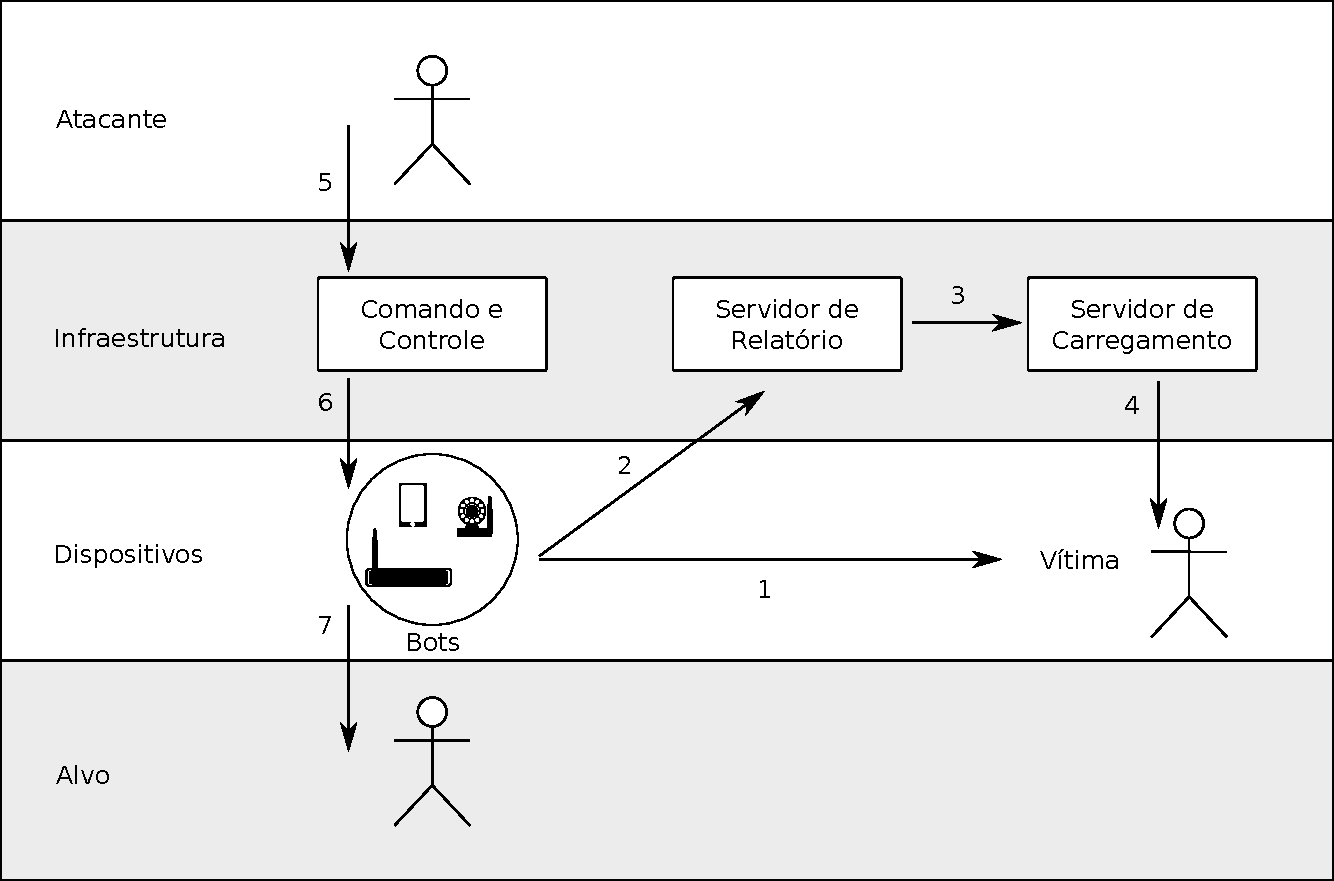
\includegraphics[width=0.7\columnwidth]{img/mirai_structure.pdf}
            \caption{Operação do Mirai.} 
            \label{fig:mirai_structure}
        \end{figure}

 
\emph{Os nossos modelos  analíticos e de  simulação focam nas contaminações dos dispositivos, ou seja, na fase de varredura (envolvendo infecções  endógenas e exógenas). Em particular, assumimos que a varredura de endereços  IPv4 pseudo-aleatórios consome recursos de banda, e que por isso a taxa de contaminações exógenas é limitada pelo \emph{poder do atacante} em função do modelo de adversário. }
    
    \textbf{Modelo de adversário}
    %    \sadoc{falar sobre adversário}
     O  adversário é o usuário que tem controle sobre o \textit{malware}. O adversário tem capacidade de reconhecer, após análise, se determinado sistema é  vulnerável, mas não é capaz de distinguir, de antemão, se determinado sistema  está, ou não, contaminado.
    Consideramos que o adversário tem uma capacidade média de contaminação exógena  de  $\Lambda$ contaminações por unidade de tempo. Essa capacidade está limitada pela taxa agregada de varredura e análise de IPs de todos os  nós que compõem a \emph{botnet}. Seja $N$ o número de nós vulneráveis na rede (ou seja, $N$ é  o número de nós que decidem não se vacinar). \emph{ No caso mais simples, supomos que a capacidade de contaminação exógena do adversário é dividida pelos nós vulneráveis presentes na rede, e que cada um é alvo de uma varredura exógena a uma taxa de  $\Lambda/N$ tentativas de contaminação por unidade de tempo.}
	
        
 